
\begin{figure}
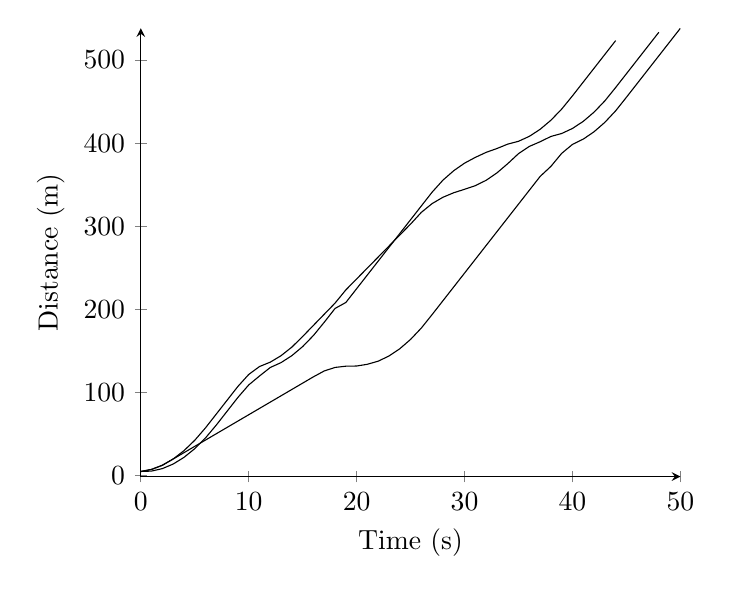
\begin{tikzpicture}
\begin{axis}[
legend style={anchor=west},
axis x line=bottom,
axis y line=left,
ymin=-1,
xlabel=Time (s),
ylabel=Distance (m),
]
\addplot[] coordinates {
(0, 5.1)
(1, 7.6)
(2, 12.6)
(3, 20.1)
(4, 30.1)
(5, 42.6)
(6, 57.6)
(7, 74.2)
(8, 90.8)
(9, 107.4)
(10, 121.758781889)
(11, 131.320742477)
(12, 136.609280481)
(13, 144.397818486)
(14, 154.68635649)
(15, 167.474894495)
(16, 180.843994592)
(17, 194.214610426)
(18, 207.587023475)
(19, 223.459436525)
(20, 236.656277515)
(21, 249.853876133)
(22, 263.052419275)
(23, 276.252160848)
(24, 289.453454774)
(25, 302.656809648)
(26, 316.797184965)
(27, 327.344349295)
(28, 334.928651733)
(29, 340.357167269)
(30, 344.481949898)
(31, 348.889623958)
(32, 355.300880372)
(33, 364.212136787)
(34, 375.302680212)
(35, 387.40549173)
(36, 396.056322381)
(37, 401.658070168)
(38, 408.039155862)
(39, 411.602111977)
(40, 417.665068092)
(41, 426.228024207)
(42, 437.290980322)
(43, 450.853936437)
(44, 466.916892552)
(45, 483.516892552)
(46, 500.116892552)
(47, 516.716892552)
(48, 533.316892552)
};
\addplot[] coordinates {
(0, 5.1)
(1, 7.6)
(2, 12.6)
(3, 20.1)
(4, 27.7044993246)
(5, 35.309054708)
(6, 42.9136778581)
(7, 50.5183839896)
(8, 58.1231932444)
(9, 65.7281328637)
(10, 73.3332406231)
(11, 80.9385704767)
(12, 88.5442022768)
(13, 96.1502594739)
(14, 103.75694369)
(15, 111.364608572)
(16, 118.973937625)
(17, 126.008316158)
(18, 130.228684814)
(19, 131.744408697)
(20, 131.932899537)
(21, 134.059124294)
(22, 137.78386123)
(23, 144.008598166)
(24, 152.733335101)
(25, 163.958072037)
(26, 177.682808973)
(27, 193.907545909)
(28, 210.507545909)
(29, 227.107545909)
(30, 243.707545909)
(31, 260.307545909)
(32, 276.907545909)
(33, 293.507545909)
(34, 310.107545909)
(35, 326.707545909)
(36, 343.307545909)
(37, 359.907545909)
(38, 372.047545909)
(39, 387.723095477)
(40, 398.507697179)
(41, 404.848995079)
(42, 413.690292979)
(43, 425.031590879)
(44, 438.872888779)
(45, 455.214186679)
(46, 471.814186679)
(47, 488.414186679)
(48, 505.014186679)
(49, 521.614186679)
(50, 538.214186679)
};
\addplot[] coordinates {
(0, 5.1)
(1, 5.58074069841)
(2, 8.56148139682)
(3, 14.0422220952)
(4, 22.0229627936)
(5, 32.503703492)
(6, 45.4844441904)
(7, 60.9651848889)
(8, 77.5651848889)
(9, 94.1651848889)
(10, 109.155902316)
(11, 119.932091931)
(12, 130.183088726)
(13, 136.060922505)
(14, 144.438756285)
(15, 155.316590064)
(16, 168.694423844)
(17, 184.572257623)
(18, 201.172257623)
(19, 208.332257623)
(20, 224.932257623)
(21, 241.532257623)
(22, 258.132257623)
(23, 274.732257623)
(24, 291.332257623)
(25, 307.932257623)
(26, 324.532257623)
(27, 341.132257623)
(28, 355.510923436)
(29, 366.882902669)
(30, 375.940014566)
(31, 382.87622765)
(32, 388.92411128)
(33, 393.530174156)
(34, 398.805256796)
(35, 402.238014529)
(36, 408.170772262)
(37, 416.603529995)
(38, 427.536287728)
(39, 440.969045461)
(40, 456.901803194)
(41, 473.501803194)
(42, 490.101803194)
(43, 506.701803194)
(44, 523.301803194)
};

\end{axis}
\end{tikzpicture}
\label{tik:100:65}
\caption{100 percent diving with GSC on route $65$}
\end{figure}
